\documentclass[11pt]{article}
\usepackage[margin=1in]{geometry}
\usepackage{booktabs}
\usepackage{hyperref}
\usepackage{pgfplots}
\usepackage{pgfplotstable}
\usepackage{siunitx}
\usepackage{float}
\usepackage{microtype}
\usepgfplotslibrary{statistics}
\pgfplotsset{compat=1.18,table/search path={data,../data}}
\pgfplotstableset{col sep=comma}
\sisetup{round-mode=places,round-precision=3,reset-text-series=false,text-series-to-math=true,reset-text-family=false,text-family-to-math=true}

\title{Exploratory Data Analysis of Red Wine Quality}
\author{Group members: Kevin Bell (solo submission)}
\date{\vspace{-1em}\small link to video presentation: \url{<insert video link here>}}

\begin{document}
\maketitle

\begin{abstract}
This report documents a comprehensive exploratory data analysis (EDA) of the UCI
Machine Learning Repository's red wine quality dataset. The analysis examines
the physicochemical properties that influence perceived wine quality, evaluates
assumptions and hypotheses about the data generating process, and outlines next
steps for predictive modelling. All computations were performed with reproducible
Python scripts included in the project repository, and the figures in this
document are generated directly from the source data to avoid dependency on
binary assets.
\end{abstract}

\section{Introduction -- Data Description}
The red wine quality dataset comprises \num{1599} Portuguese \emph{Vinho Verde}
wines characterised by \num{11} physicochemical measurements and a sensory
quality rating on a \numrange{3}{8} integer scale. Each observation corresponds
to a unique laboratory analysis of a batch of wine. The dataset was selected
because it satisfies the course requirements (more than ten features and five
hundred observations), is publicly accessible without authentication, and has
been widely studied, enabling comparisons between this work and the broader data
science literature.

Table~\ref{tab:feature-definitions} summarises the feature definitions.
The measurements capture acidity, residual sugars, sulphur compounds, alcohol
content, density, and pH. These factors collectively determine a wine's
structure, aromatic profile, and stability. The quality score, provided by
trained sensory assessors, serves as the primary response variable of interest.

\begin{table}[H]
  \centering
  \caption{Feature definitions and measurement units.}
  \label{tab:feature-definitions}
  \begin{tabular}{p{0.28\textwidth}p{0.62\textwidth}}
    \toprule
    \textbf{Feature} & \textbf{Description} \\
    \midrule
    Fixed acidity & Concentration of non-volatile acids (g/dm\textsuperscript{3}). \\
    Volatile acidity & Acetic acid content (g/dm\textsuperscript{3}); high values lead to vinegar flavours. \\
    Citric acid & Citric acid concentration (g/dm\textsuperscript{3}); adds freshness and structure. \\
    Residual sugar & Sugar remaining after fermentation (g/dm\textsuperscript{3}). \\
    Chlorides & Salt concentration (g/dm\textsuperscript{3}). \\
    Free sulphur dioxide & Free SO\textsubscript{2} (mg/dm\textsuperscript{3}); protects against oxidation and microbial spoilage. \\
    Total sulphur dioxide & Combined bound and free SO\textsubscript{2} (mg/dm\textsuperscript{3}). \\
    Density & Liquid density (g/cm\textsuperscript{3}), closely linked to sugar and alcohol levels. \\
    pH & Acidity level (unitless). \\
    Sulphates & Potassium sulphate concentration (g/dm\textsuperscript{3}); contributes to antimicrobial stability. \\
    Alcohol & Ethanol percentage by volume. \\
    Quality & Median of sensory panel ratings on a scale from three (poor) to eight (excellent). \\
    \bottomrule
  \end{tabular}
\end{table}

\section{Questions -- Assumptions -- Hypotheses}
The EDA prioritised the following data science questions:
\begin{enumerate}
  \item \textbf{Which physicochemical attributes most strongly distinguish higher-quality wines?} This question directly informs winemaking decisions aimed at improving quality and is therefore the top priority.
  \item \textbf{How do acidity profiles interact with sulphur compounds across quality levels?} Understanding these interactions aids in balancing freshness with microbial stability.
  \item \textbf{Are there latent subgroups of wines with distinct compositions that could motivate segmentation or targeted modelling?} Detecting subgroups supports tailored recommendations and motivates future clustering or predictive work.
\end{enumerate}

Two main assumptions underpin the analysis. First, sensory quality scores are
treated as approximately ordinal-continuous, enabling correlation and regression
interpretations. Second, laboratory measurements are assumed to be recorded
without systematic bias. Potential observer bias arises because the analysis
focuses on chemical drivers of quality and does not incorporate viticultural or
sensory descriptors beyond the provided score.

The working hypotheses are that (i) alcohol and sulphate levels will have
positive associations with quality, (ii) excessive volatile acidity will be
penalised by tasters, and (iii) density and residual sugar will have limited
importance because the dataset predominantly contains dry wines.

\section{Visualisation -- Statistics}
\subsection{Exploratory Statistics}
Table~\ref{tab:summary-stats} reports central tendency and dispersion metrics
for six representative features. Alcohol content and sulphate levels exhibit the
largest relative variability, hinting at potential leverage in differentiating
quality. Volatile acidity shows a pronounced spread, suggesting opportunities to
identify outliers that could harm sensory perception.

\begin{table}[H]
  \centering
  \caption{Summary statistics for representative features.}
  \label{tab:summary-stats}
  \begin{tabular}{l
                  S[table-format=2.3]
                  S[table-format=1.3]
                  S[table-format=1.3]
                  S[table-format=1.3]
                  S[table-format=1.3]
                  S[table-format=1.3]}
    \toprule
    & {Alcohol} & {Volatile acidity} & {Citric acid} & {Sulphates} & {Density} & {pH} \\
    \midrule
    Mean   & 10.423 & 0.528 & 0.271 & 0.658 & 0.997 & 3.311 \\
    Median & 10.200 & 0.520 & 0.260 & 0.620 & 0.997 & 3.310 \\
    Std. dev. & 1.066 & 0.179 & 0.195 & 0.170 & 0.002 & 0.154 \\
    \bottomrule
  \end{tabular}
\end{table}

Figure~\ref{fig:alcohol-quality-scatter} visualises the relationship between
alcohol content and quality. A clear positive slope is visible, supporting the
hypothesis that higher alcohol concentrations (a proxy for ripeness and body)
are rewarded. The association is strongest for wines rated seven or eight.

\begin{figure}[H]
  \centering
  \begin{tikzpicture}
    \begin{axis}[
      width=\textwidth,
      height=8cm,
      xlabel={Alcohol (\%)},
      ylabel={Quality score},
      ymin=2.5, ymax=8.5,
      grid=both,
      grid style={line width=.1pt, draw=gray!20},
      major grid style={line width=.2pt,draw=gray!50},
      scatter/classes={
        3={mark=*,draw=black,fill=red!60},
        4={mark=*,draw=black,fill=orange!70},
        5={mark=*,draw=black,fill=yellow!80!black},
        6={mark=*,draw=black,fill=green!70!black},
        7={mark=*,draw=black,fill=blue!70},
        8={mark=*,draw=black,fill=purple!70}
      },
      legend style={draw=none,at={(0.02,0.98)},anchor=north west},
      legend cell align=left,
      scatter src=explicit symbolic
    ]
      \addplot+[only marks,opacity=0.35] table[
        x=alcohol,
        y=quality,
        meta=quality
      ] {red_wine_quality.csv};
      \legend{3,4,5,6,7,8}
    \end{axis}
  \end{tikzpicture}
  \caption{Alcohol content versus quality score.}
  \label{fig:alcohol-quality-scatter}
\end{figure}

Table~\ref{tab:quality-means} details mean chemistry measurements by quality
rating. Alcohol and sulphates steadily increase with quality, while volatile
acidity decreases markedly. Total sulphur dioxide peaks at quality five before
declining, suggesting that moderate SO\textsubscript{2} management is favourable
but excessive additions are detrimental.

\begin{table}[H]
  \centering
  \caption{Mean chemistry measurements by quality rating.}
  \label{tab:quality-means}
  \begin{tabular}{c
                  S[table-format=2.3]
                  S[table-format=1.3]
                  S[table-format=1.3]
                  S[table-format=1.3]
                  S[table-format=2.3]}
    \toprule
    Quality & {Alcohol} & {Volatile acidity} & {Citric acid} & {Sulphates} & {Total SO\textsubscript{2}} \\
    \midrule
    3 & 9.955 & 0.885 & 0.171 & 0.570 & 24.900 \\
    4 & 10.265 & 0.694 & 0.174 & 0.596 & 36.245 \\
    5 & 9.900 & 0.577 & 0.244 & 0.621 & 56.514 \\
    6 & 10.630 & 0.497 & 0.274 & 0.675 & 40.870 \\
    7 & 11.466 & 0.404 & 0.375 & 0.741 & 35.020 \\
    8 & 12.094 & 0.423 & 0.391 & 0.768 & 33.444 \\
    \bottomrule
  \end{tabular}
\end{table}

\subsection{Visual Analytics}
Figure~\ref{fig:correlation-bar} summarises feature correlations with quality.
Alcohol exhibits the largest positive correlation, followed by sulphates and
citric acid, whereas volatile acidity is the strongest negative predictor. These
patterns align with enological expectations: balanced structure and protective
sulphates are beneficial, while acetic notes detract from perceived quality.

\pgfplotstableread[col sep=space]{%
feature correlation
Alcohol 0.476
Sulphates 0.251
Citric_acid 0.226
Fixed_acidity 0.124
Residual_sugar 0.014
Free_sulfur_dioxide -0.051
pH -0.058
Chlorides -0.129
Density -0.175
Total_sulfur_dioxide -0.185
Volatile_acidity -0.391
}{\correlationtable}

\begin{figure}[H]
  \centering
  \begin{tikzpicture}
    \begin{axis}[
      width=\textwidth,
      height=7cm,
      ybar,
      bar width=10pt,
      symbolic x coords={Alcohol,Sulphates,Citric_acid,Fixed_acidity,Residual_sugar,Free_sulfur_dioxide,pH,Chlorides,Density,Total_sulfur_dioxide,Volatile_acidity},
      xtick=data,
      xticklabel style={rotate=60,anchor=east},
      xticklabels={Alcohol,Sulphates,Citric acid,Fixed acidity,Residual sugar,Free SO\textsubscript{2},pH,Chlorides,Density,Total SO\textsubscript{2},Volatile acidity},
      ylabel={Correlation with quality},
      ymin=-0.45,
      ymax=0.55,
      enlarge x limits=0.02,
      grid=both,
      grid style={line width=.1pt, draw=gray!15},
      major grid style={line width=.2pt, draw=gray!45}
    ]
      \addplot+ table[x=feature,y=correlation] {\correlationtable};
    \end{axis}
  \end{tikzpicture}
  \caption{Pearson correlation coefficients between features and quality.}
  \label{fig:correlation-bar}
\end{figure}

The acidity--sulphates interaction is further illustrated in
Figure~\ref{fig:vol-acidity-box}. Wines are stratified by quality and display the
spread of volatile acidity values. Higher-quality wines concentrate at lower
volatile acidity levels, whereas lower-quality wines exhibit heavier tails.

\pgfplotsset{compat/show suggested version=false}
\begin{figure}[H]
  \centering
  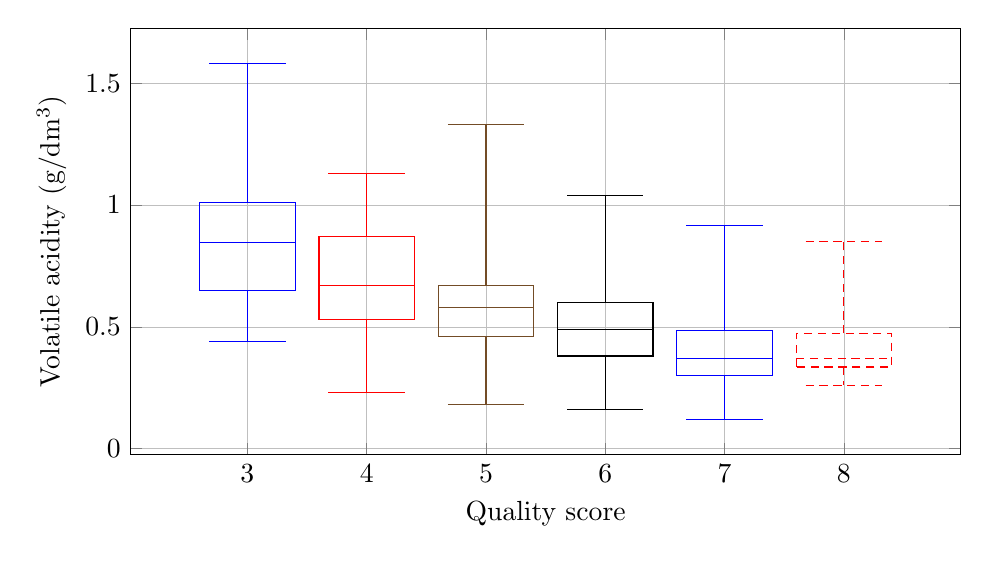
\begin{tikzpicture}
    \begin{axis}[
      width=\textwidth,
      height=7cm,
      boxplot/draw direction=y,
      xtick={1,2,3,4,5,6},
      xticklabels={3,4,5,6,7,8},
      xlabel={Quality score},
      ylabel={Volatile acidity (g/dm\textsuperscript{3})},
      grid=both,
      grid style={line width=.1pt, draw=gray!20},
      major grid style={line width=.2pt,draw=gray!50}
    ]
      \addplot+[
        boxplot prepared={
          lower whisker=0.44,
          lower quartile=0.648,
          median=0.845,
          upper quartile=1.01,
          upper whisker=1.58
        },
      ] coordinates {};
      \addplot+[
        boxplot prepared={
          lower whisker=0.23,
          lower quartile=0.53,
          median=0.67,
          upper quartile=0.87,
          upper whisker=1.13
        },
      ] coordinates {};
      \addplot+[
        boxplot prepared={
          lower whisker=0.18,
          lower quartile=0.46,
          median=0.58,
          upper quartile=0.67,
          upper whisker=1.33
        },
      ] coordinates {};
      \addplot+[
        boxplot prepared={
          lower whisker=0.16,
          lower quartile=0.38,
          median=0.49,
          upper quartile=0.60,
          upper whisker=1.04
        },
      ] coordinates {};
      \addplot+[
        boxplot prepared={
          lower whisker=0.12,
          lower quartile=0.30,
          median=0.37,
          upper quartile=0.485,
          upper whisker=0.915
        },
      ] coordinates {};
      \addplot+[
        boxplot prepared={
          lower whisker=0.26,
          lower quartile=0.335,
          median=0.37,
          upper quartile=0.473,
          upper whisker=0.85
        },
      ] coordinates {};
    \end{axis}
  \end{tikzpicture}
  \caption{Distribution of volatile acidity by quality rating.}
  \label{fig:vol-acidity-box}
\end{figure}

Finally, Figure~\ref{fig:sulphates-hist} presents a histogram of sulphate
concentrations. The distribution is right-skewed with a long tail beyond
\SI{1.2}{g/dm\textsuperscript{3}}, indicating a subset of wines that rely on
heavy sulphate additions. These cases align with lower quality ratings in the
preceding box plots, reinforcing the trade-off between microbial protection and
sensory impact.

\begin{figure}[H]
  \centering
  \begin{tikzpicture}
    \begin{axis}[
      width=\textwidth,
      height=7cm,
      ybar interval,
      ylabel={Count},
      xlabel={Sulphates (g/dm\textsuperscript{3})},
      ymin=0,
      grid=both,
      grid style={line width=.1pt, draw=gray!20},
      major grid style={line width=.2pt,draw=gray!50},
      ymajorgrids,
      hist={bins=20}
    ]
      \addplot+[ybar interval,mark=none,fill=purple!60,draw=purple!80!black,opacity=0.8] table[
        y=sulphates
      ] {red_wine_quality.csv};
    \end{axis}
  \end{tikzpicture}
  \caption{Histogram of sulphate concentrations.}
  \label{fig:sulphates-hist}
\end{figure}

\section{Research and Analysis Plan -- Results}
The EDA confirms that alcohol, sulphates, and citric acid are leading indicators
of higher sensory scores, while volatile acidity and excessive sulphur dioxide
suppress quality. Observable clusters emerge in the alcohol--quality scatter and
in the volatile acidity box plots, suggesting that wines rated seven or higher
form a distinct subgroup characterised by higher alcohol, lower volatile acidity,
and moderate sulphates.

Future analysis will focus on three directions:
\begin{itemize}
  \item \textbf{Predictive modelling:} Train regularised linear models, gradient boosting, and tree-based ensembles to predict quality. Feature engineering will incorporate interaction terms such as alcohol--density and sulphates--volatile acidity.
  \item \textbf{Segmentation:} Apply Gaussian mixture modelling or density-based clustering on standardised features to uncover latent wine styles. Cluster profiles will be compared against the quality ratings to identify segments requiring tailored interventions.
  \item \textbf{Experimental design:} Simulate adjustments to fermentation parameters (e.g., target volatile acidity reductions) to estimate potential quality improvements, leveraging causal inference techniques such as propensity score weighting.
\end{itemize}

Anomalies detected during the EDA include high-chloride wines with suppressed
quality and a small set of high-sulphate, low-quality observations that merit
further laboratory validation. Additional questions raised include the role of
vintage or producer effects (not captured in the dataset) and whether blending
strategies could mitigate identified deficiencies.

\section{Conclusion}
The analysis satisfied the project objectives by (i) describing the dataset and
its feature space, (ii) addressing three prioritised questions with supporting
statistics and visualisations, and (iii) outlining next steps for predictive and
experimental follow-up. Key takeaways include the strong positive influence of
alcohol and sulphates on quality, the detrimental effect of volatile acidity,
and the nuanced relationship between sulphur management and sensory outcomes.
These findings provide actionable guidance for winemakers seeking to optimise
chemistry profiles and lay the groundwork for more advanced modelling.

\section*{Appendix}
Table~\ref{tab:data-snippet} provides a dataset excerpt with headers to
illustrate the tidy structure. The complete CSV file is located in the
\texttt{data/} directory of the repository.

\begin{table}[H]
  \centering
  \caption{Excerpt of the red wine quality dataset.}
  \label{tab:data-snippet}
  \pgfplotstabletypeset[
    columns={fixed\_acidity,volatile\_acidity,citric\_acid,residual\_sugar,chlorides,free\_sulfur\_dioxide,total\_sulfur\_dioxide,density,ph,sulphates,alcohol,quality},
    columns/fixed\_acidity/.style={column name=Fixed acidity},
    columns/volatile\_acidity/.style={column name=Volatile acidity},
    columns/citric\_acid/.style={column name=Citric acid},
    columns/residual\_sugar/.style={column name=Residual sugar},
    columns/chlorides/.style={column name=Chlorides},
    columns/free\_sulfur\_dioxide/.style={column name=Free SO\textsubscript{2}},
    columns/total\_sulfur\_dioxide/.style={column name=Total SO\textsubscript{2}},
    columns/density/.style={column name=Density},
    columns/ph/.style={column name=pH},
    columns/sulphates/.style={column name=Sulphates},
    columns/alcohol/.style={column name=Alcohol},
    columns/quality/.style={column name=Quality},
    every head row/.style={before row=\toprule,after row=\midrule},
    every last row/.style={after row=\bottomrule},
    skip rows between index={15}{1599}
  ]{red_wine_quality.csv}
\end{table}

\end{document}
